\documentclass[11pt]{article}
\usepackage[margin=0.8in]{geometry}
\usepackage{amsmath}
\usepackage[dvipsnames]{xcolor}
\usepackage{graphicx}
\usepackage{hyperref}
\usepackage{mathtools}
\usepackage{tikz,graphics,color,fullpage,float,epsf,caption,subcaption}
\DeclarePairedDelimiter{\floor}{\lfloor}{\rfloor}

\usepackage[noend]{algpseudocode}

\newcommand{\ggets}{\gets}


​
​
\title{CS3510-A: Design and Analysis of Algorithms, Spring 2021} 
​
\author{Homework-5}
​
\begin{document}
% \maketitle
\begin{center}
    
    \LARGE CS3510-A: Design and Analysis of Algorithms, Spring 2021 \\ \vspace{1em} 
    \large Homework-5 \\ \vspace{0.5em}
    February 16, 2021
\end{center}
\thispagestyle{empty}
\pagestyle{empty}
​
\noindent
\begin{center}
{\bf DUE DATE: Tuesday, February 23, 1l:59pm}
\end{center}
​
\noindent
{\bf Note-1:} Your homework solutions should be electronically formatted as a single PDF document that you will upload on Gradescope. 
If you have to include some handwritten parts, please make sure that they are very clearly written and that you include them as high resolution images. \\
​
\noindent
{\bf Note-2:} Please think twice before you copy a solution from another student or resource (book, web site, etc). 
It is not worth the risk and embarrassment. \\
​
\noindent
{\bf Note-3:} You need to {\bf explain/justify} your answers. Do not expect full credit if you just state the correct answer. \\
​
\noindent
{\bf Note-4: You will get 2 extra points if you submit electronically typed solutions instead of hand-written.} 
​
\newpage
\section*{Problem-1 (30 points)}
A binary tree is called “complete” if (1) every internal node has two children, and (2) every leaf node has the same depth (distance from the root). 


Describe a divide-and-conquer algorithm that computes the largest complete subtree T* of a given binary tree T. The algorithm should return both the root and the depth of T*. Note that the leaves of T* may not be leaves in the T (i.e., T* may be “internal” in T).
Also analyze the run time of your algorithm.


\subsection*{Solution}
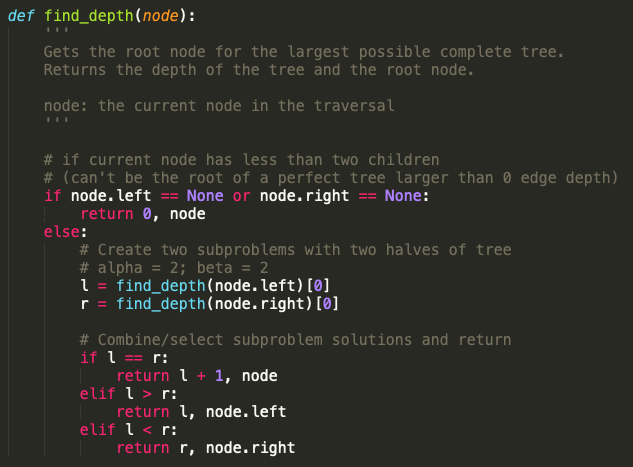
\includegraphics[scale=0.5]{tree.png}

\subsection*{Explanation}
The algorithm starts the recursive solution at the root node for the whole tree. If a node has $<2$ child nodes then it is a base case and ($0, curr$) is returned as the solution for the subproblem. If the current node has two children then two subproblems are created, one for each child node. This results in two subproblems with size $n/2$. Once the solutions two the two subproblems are found they are "combined". If the two solutions return an identical depth, then they can become two symmetrical halves with the current node as the new root (solution is $(l+1, curr)$). If one subproblem's solution is larger than the other's solution, then that $(depth, node)$ solution gets passed up to the parent call until a larger tree can be made. This combination of solutions can be done in $O(1)$.

\subsection*{Runtime}
General runtime for this algo:\\
$T(n) = 2T(n/2) + O(1)$\\

\noindent For the master theorem, the values are:\\
\noindent $\alpha=2$: because each call of the function results in two recursive subcalls.\\
$\beta=2$: because the size of the tree for each subcall call will be at most of size $n/2$.\\
$\gamma=0$: because the work of verifying the solution is $O(1)$, meaning for $O(n^\gamma)$, $\gamma = 0$.\\

\noindent In this case: $\gamma < \log_\beta \alpha$ $(0 < \log_2 2)$\\
Therefore this algorithm has: $O(n^\log_2 2)$ or $O(n)$.



​
\newpage
\section*{Problem-2 (35 points)}
\noindent
Suppose that we have two sorted lists $a$ and $b$. The size of $a$ is $n$ entries and the size of $b$ is $m$ entries. Design an algorithm to find the $k$’th smallest element in the union of $a$ and $b$ in $O(log(n+m))$ time. Please also analyze the run time of your algorithm.


\subsection*{Solution}
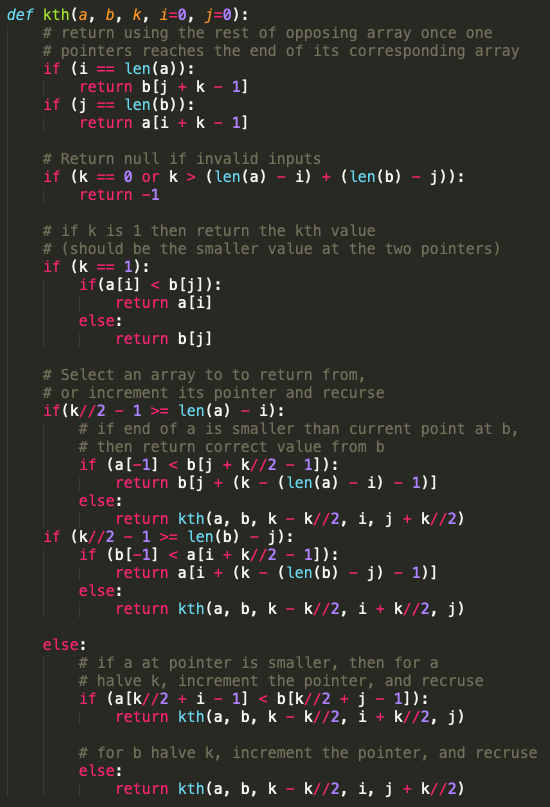
\includegraphics[scale=0.5]{kth.png}

\subsection*{Explanation}
By using a pointer for each array and recursively incrementing pointers by half of k and recursively halving k, the algorithm essentially performs a binary search over both arrays at once. The algorithm has several checks to the behavior of having two pointers. If one pointer reaches the end of its array then the corresponding value at the pointer in the other array will be returned. If no value can be returned, then the pointer for either array will be incremented by $k/2$ and $k$ will decrease by $k/2$. This recursion results in at most one subcall for any call to the function and moving the pointers eliminates at most half the total values in all arrays. "Combining" the solution from a subcall is done by simply retuning the result to the parent call, therefore combining results can be done in $O(1)$.

\subsection*{Runtime}
General runtime for this algo:\\
$T(n) = T(n/2) + O(1)$\\

\noindent For the master theorem, the values are:\\
\noindent $\alpha=1$: because each call of the function results in only one recursive call.\\
$\beta=2$: because the total number of values considered by the algo decreases by $n/2$ for each subcall\\
$\gamma=0$: because the "combination" of results can be done in $O(1)$, meaning for $O(n^\gamma)$, $\gamma = 0$\\

\noindent In this case: $\gamma = \log_\beta \alpha$ $(0 = \log_2 1)$\\
Therefore this algorithm has: $O(\log n$), but in this case $n$ is the total number of values in both arrays so the real runtime is $O(\log(n+m))$.


\newpage
\section*{Problem-3 (35 points)}
You are given $n$ non-vertical lines in the plane, labeled $L_1, ..., L_n$ , with the $i$'th line specified by the equation $y = a_i*x + b_i$ . We will make the assumption that no three of these lines  meet at a single point and these lines extend infinitely. 


We say that line $L_i$ is {\bf uppermost at a given
x-coordinate $x_0$} if its y-coordinate at $x_0$ is greater than the y-coordinates
of all the other lines at $x_0$ : $a_i*x_0 + b_i > a_j * x_0 + b_j$ for all $j \neq i$. 


We say that line $L_i$ is
{\bf visible} if there is some x-coordinate at which $L_i$ is uppermost.
Intuitively,
some portion of $L_i$ can be "seen" if you look down from $y = +\infty$.


Design an algorithm that takes $n$ lines as input and in $O(n \log{n})$ time
returns the set of lines that are visible. Fig. \ref{Fig1} gives an example. 

Please also analyze the run time of your algorithm.


\noindent
\textbf{Note:} Make sure that your solution uses the divide-and-conquer approach. \\
\textbf{Hint:} You can first sort all lines by their slopes, and then split the problem. \\




\begin{figure}[H]
\centering
\includegraphics[width=0.7\textwidth]{hw5/hw5_p3.jpeg} 
\caption{All the lines except for 2 are visible.}
\label{Fig1} 
\end{figure}
 
 

\subsection*{Solution}

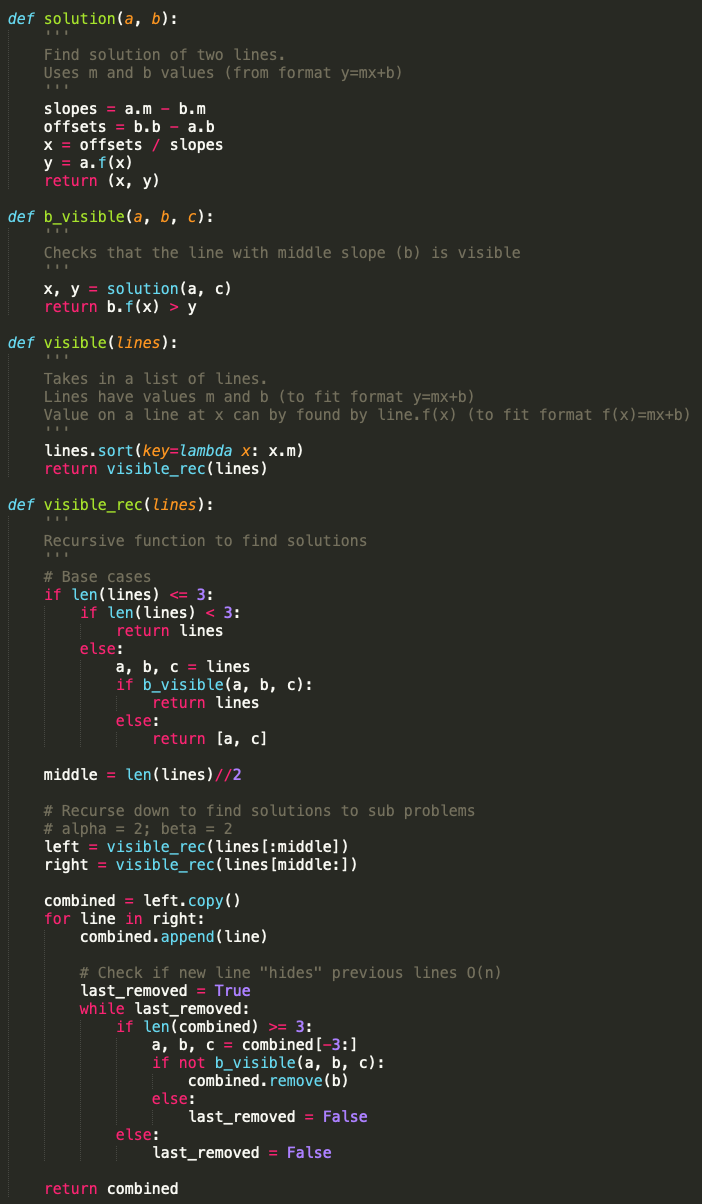
\includegraphics[scale=0.4]{code.png}

\subsection*{Explanation}
The algorithm sorts the list of lines by slope. The algorithm then recursively splits the list of lines into two lists, split at the middle of the list (two groups of size n/2). Once the recursive function receives a list with length $\leq{3}$ if length $\leq{2}$, then the algo returns the list. If length $=3$ then the function checks that median line (by slope) is visible ($f(x)$ for the median line is greater than the $f(x)$ for the other lines where $x$ is the intersection of the other two lines). Finding the intersection of two lines and checking the visibility of the median line in a list of three sorted lines can both be done in $O(1)$. Once two subproblems have been solved the algorithm combines two solutions by iteratively adding solutions from the "right" (higher slope) side to solutions from the "left" (lower slope) side, while checking if newly added lines will "hide" existing lines in the larger solution. If an existing line in the combined solution is hidden by the newly added line then the hidden line will be removed from the solution. This combination of solutions for subproblems can be done in $O(n)$.

\subsection*{Runtime}
General runtime for this algo:\\
$T(n) = 2T(n/2) + O(n)$\\

\noindent For the master theorem, the values are:\\
\noindent $\alpha=2$: because each call that is not a base case will result in the creation of two subproblems.\\
$\beta=2$: because the input size for each subproblem will be $n/2$.\\
$\gamma=1$: because combining suproblem solutions can be done in $O(n)$, meaning for $O(n^\gamma), \gamma=1$\\

\noindent In this case: $\gamma = \log_\beta \alpha$ $(1 = \log_2 2)$\\
Therefore this algorithm has: $O(n \log n)$


\end{document}